\documentclass[utf8, aspectratio=169]{beamer}

% \usepackage{fontspec}
\usepackage{tikz}
\usetikzlibrary{automata, positioning, arrows, calc}
\usepgflibrary{fpu}
\pgfdeclarelayer{bg}    % declare background layer
\pgfsetlayers{bg,main}

\usepackage{amsmath}
\DeclareMathOperator{\pgkd}{pgkd}

\setbeamercolor{notebox}{bg=structure.fg!20!white}

\AtBeginSection[] % Do nothing for \section*
{
 \begin{frame}<beamer>
   \frametitle{Superrigardo}
   \tableofcontents[currentsection]
 \end{frame}
}

\title{Postkvantuma ĉifrado}
\author{Johannes Mueller}
\institute{KAEST 2024 – Žilina}
\date{8a de Novembro 2024}


\begin{document}

\begin{frame}
  \titlepage
\end{frame}

\begin{frame}
  \frametitle{Superrigardo}
  \tableofcontents
\end{frame}

\section{Enkonduko}

\begin{frame}
  \frametitle{La aspektoj de datuma sekureco}

  Ekzistas tri bazaj aspektoj de datuma sekureco

  \begin{description}
  \item<2->[konfidenteco] {\color<6->{green!50!black} neniu necelata povas legi la datumojn}
  \item<3->[fidindeco] {\color<6->{green!50!black} pruveblo de la deveno kaj la aŭtenteco}
  \item<4->[disponeblo] {\color<6->{gray} datumoj estas disponebla kiam bezonataj}
  \end{description}

  \vspace{1em}
  \uncover<5->{Ĉiuj tri estas grava parto de la nuntempa ĉiutaga vivo.}
\end{frame}

\begin{frame}
  \frametitle{Terminologio}
  \begin{description}
  \item[klarmesaĝo] la neĉifrita mesaĝo
  \item[ĉifraĵo] la ĉifrita mesaĝo
  \item[ĉifri] transformi klarmesaĝon al ĉifraĵo per ŝlosilo
  \item[malĉifri] transformi ĉifraĵon al klarmesaĝo per ŝlosilo
  \item[ŝlosilo] datumo por ĉifri aŭ malĉifri mesaĝon
  \item[haketo] testsumo por pruvi ĉu mesaĝo estas aŭtenta
  \item[subskribo] pruvilo ke mesaĝo kaj la deveno estas aŭtentaj
  \end{description}
\end{frame}


\section{Klasika ĉifrado}

\begin{frame}
  \frametitle{La principoj de Kerckoff}
  La principoj de Kerckoff (1883):
  \begin{itemize}
  \item<alert@2> La sistemo ne estu sekreta (nur la ŝlosilo).
  \item La ĉifraĵo ne estu distingebla de hazarda datumo.
  \item La ĉifraĵo estu transsendebla elektronike.
  \item La sistemo estu transportebla kaj uzebla pere de unu persono.
  \item La sistemo estu facile uzebla.
  \end{itemize}
\end{frame}

\begin{frame}
  \frametitle{Simetria ĉifrado}
  \begin{figure}
    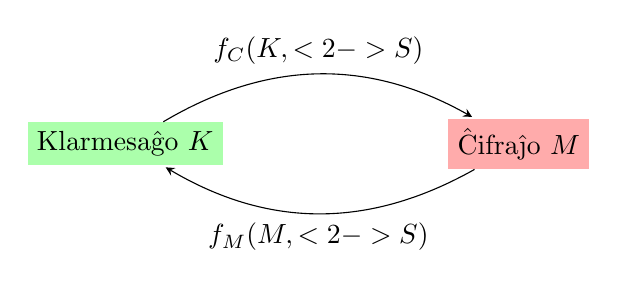
\begin{tikzpicture}[
      ->,>=stealth,shorten >=1pt,
      auto,
      node distance=5cm,
      ]
      \node [fill=green!33] (km) {Klarmesaĝo $K$};
      \node [fill=red!33, right of=km] (cf) {Ĉifraĵo $M$};

      \draw (km) edge[bend left] node {$f_C(K, \alert<2->{S})$} (cf);
      \draw (cf) edge[bend left] node {$f_M(M, \alert<2->{S})$} (km);
    \end{tikzpicture}
  \end{figure}

  \begin{itemize}
  \item $f_c(K, \alert<2->{S}) = M$
  \item $f_M(M, \alert<2->{S}) = K$
  \item<2-> \alert{$S$} estas la ŝlosilo por ĉifri kaj malĉifri
  \end{itemize}

  \uncover<3->{%
    \begin{beamercolorbox}[center, rounded=true, shadow=true]{notebox}
      \textbf{Malavantaĝo:} interŝanĝo de la ŝlosilo malsekura
    \end{beamercolorbox}
  }
\end{frame}

\begin{frame}
  \frametitle{Malsimetria ĉifrado}
  \begin{figure}
  \begin{tikzpicture}[node distance=0.5em,align=left]

    \node (anjo) at (0,0) {Anjo};
    \node (boĉjo) at (6,0) {Boĉjo};
    \node (publika) at ($(anjo)!0.5!(boĉjo)$) {publiko};

    \node [below=of anjo] (priv) {{\uncover<2->{\color<10->{red}$S_{priv}$}}};
    \node [below=of priv] (pub_a) {{\uncover<3->{$\textcolor<11->{green!70!black}{S_{pub}} = P({\color<10->{red}S_{priv}})$}}};
    \node (pub_b) at (pub_a -| boĉjo) {{\uncover<5->{$\color<11->{green!70!black}S_{pub}$}}};
    \node (pub) at ($(pub_a)!0.5!(pub_b)$) {{\uncover<4->{$\color<11->{green!70!black}S_{pub}$}}};

    \uncover<4->{\draw[->] (pub_a) -- (pub);}

    \uncover<5->{\draw[->] (pub) -- (pub_b);}


    \node [below=of pub_b] (klar) {{\uncover<6->{$K$}}};

    \node [below=of klar] (cf_b) {{\uncover<7->{$M = f_C(K, \textcolor<11->{green!70!black}{S_{pub}})$}}};

    \node (cf_a) at (cf_b -| anjo) {{\uncover<8->{$M$}}};
    \uncover<8->{\draw[->] (cf_b) -- (cf_a);}

    \node [below=of cf_a] (mcf) {{\uncover<9->{$K = f_M(M, {\color<10->{red}S_{priv}})$}}};

    \begin{pgfonlayer}{bg}
      \fill [fill=red!20]
      ($(anjo) + (-4em,2em)$) rectangle ($(mcf) + (4em, -2em)$) coordinate (anjo border);

      \fill [fill=green!20]
      (anjo border) rectangle ($(boĉjo) + (-4em, 2em)$) coordinate (boĉjo border);

      \fill [fill=magenta!20]
      ($(boĉjo) + (4em, 2em)$) rectangle (anjo border -| boĉjo border);
    \end{pgfonlayer}

  \end{tikzpicture}
\end{figure}

\end{frame}

\begin{frame}
  \frametitle{Unudirekta funkcio}
  \[ S_{pub} = P(S_{priv}) \; \longleftarrow \text{facile}\]
  \[ S_{priv} = P_i(S_{pub}) \; \longleftarrow \text{malfacile}\]

  \pause
  \vspace{1em}
  Ekzemple produkto de du primoj:

  \pause
  \begin{itemize}
  \item $23 \times 37 = 851$ unu multobligo
  \item $851 = ? \times ?$ multaj provoj
  \item $1475707273*6077236961 = 8968222783092117353$
  \end{itemize}

  \pause
  La komplekseco de $P_i$ kreskas pli rapide ol tiu de $P$

  \pause
  \vspace{0.5em}
  Rekordo: En 2020 oni faktorigis 250-ciferan (829bit) nombron en 2700
  procesilaj horoj de Intel Xeon Gold 6130 at 2.1 GHz.

  \vspace{0.5em}
  Kutimaj ŝlosiloj uzas 2048 aŭ 4096 bitojn.
\end{frame}

\begin{frame}
  \frametitle{Sekureco de unudirektaj funkcioj}
  \begin{columns}
    \begin{column}{0.5\textwidth}
      Tri unudirektaj funkcioj en uzo
      \begin{itemize}
      \item faktorigo de produkto de du primoj
      \item diskreta logaritmo
      \item eliptaj kurboj
      \end{itemize}
      \uncover<2->{Ĉu ili vere estas sekuraj?}
    \end{column}
    \begin{column}{0.5\textwidth}
      \uncover<3->{\includegraphics[width=\linewidth]{peter-shor.png}}

    \end{column}
  \end{columns}
\end{frame}


\section{Minaco de kvantuma komputilado}

\begin{frame}
  \frametitle{Kvantuma komputilo}
  Klasika komputilo\par
  \begin{figure}
  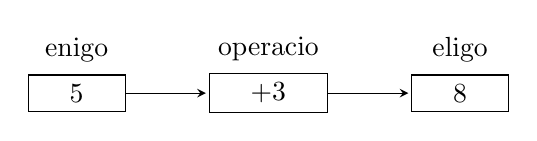
\begin{tikzpicture}[>=stealth,shorten >=1pt]
    \begin{scope}[every node/.style=draw,inner xsep=15pt]
      \node [draw] (input) {$5$};
      \node [draw, right=3em of input] (operation) {$+3$};
      \node [draw, right=3em of operation] (output) {$8$};
    \end{scope}
    \node [above=0.1em of input] {enigo};
    \node [above=0.1em of operation] {operacio};
    \node [above=0.1em of output] {eligo};

    \draw [->] (input) -- (operation);
    \draw [->] (operation) -- (output);
  \end{tikzpicture}
  \end{figure}
  \pause

  \vspace{2em}

  Kvantuma komputilo\par
  \begin{figure}
  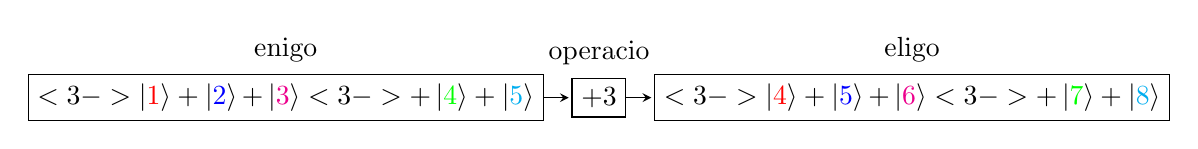
\begin{tikzpicture}[>=stealth,shorten >=1pt]
    \begin{scope}[every node/.style=draw]
      \node [draw] (input) {
        $\invisible<3->{\left|\textcolor{red}{1}\right> + \left|\textcolor{blue}{2}\right> +}
        \left|\textcolor{magenta}{3}\right>
        \invisible<3->{+ \left|\textcolor{green}{4}\right> + \left|\textcolor{cyan}{5}\right>}$
      };
      \node [draw, right=1em of input] (operation) {$+3$};
      \node [draw, right=1em of operation] (output) {
        $
        \invisible<3->{\left|\textcolor{red}{4}\right> + \left|\textcolor{blue}{5}\right> +}
        \left|\textcolor{magenta}{6}\right>
        \invisible<3->{+ \left|\textcolor{green}{7}\right> + \left|\textcolor{cyan}{8}\right>}
        $};
    \end{scope}
    \node [above=0.1em of input] {enigo};
    \node [above=0.1em of operation] {operacio};
    \node [above=0.1em of output] {eligo};

    \draw [->] (input) -- (operation);
    \draw [->] (operation) -- (output);
  \end{tikzpicture}
  \end{figure}
\end{frame}

\begin{frame}[label=shor]
  \frametitle{Algoritmo de Shor}
  \[ N = a b \;\text{kun}\; a, b \in \mathbb{N} \]
  \uncover<2->{Ni divenas $1 < d < N$, se $\pgkd(d, N) \neq 1$ → sukceso}
  \uncover<3->{\[
    \exists p  \in \mathbb{N} \left|  \right. d^p = m N + 1 \;\text{kun}\; m
    \in \mathbb{N}
  \]}%
  \uncover<4->{\[ d^p - 1 = \left(d^{p/2} + 1\right)\left(d^{p/2} - 1\right) = m N \]}

  \uncover<5->{%
    En $37,5 \%$ de la divenoj
    \begin{itemize}
    \item $p$ estas para
    \item $d^{p/2} \pm 1$ estas divizoro de $N$
    \end{itemize}
    \uncover<6>{%
      \begin{beamercolorbox}[center, rounded=true, shadow=true]{notebox}
        Kiel kalkuli $p$?
    }
    \end{beamercolorbox}
  }
\end{frame}

\begin{frame}
  \frametitle{Algoritmo de Shor – kvantuma parto}
  Kun la divenita $d$:
  \begin{figure}
  \begin{tikzpicture}[>=stealth,shorten >=1pt]
    \node [draw] (input) {
      $\left|1\right> + \left|2\right> + \left|3\right> + \left|4\right> +
      \left|5\right> + \left|6\right> + \left|7\right> + \left|8\right> + \ldots $
    } node [above=1em] {\small superpozicio de ĉiuj eblaj valoroj por $p$};
    \node [draw, below=of input.west] (step1) {$d^x$};
    \node [draw, right=of step1] (potential) {
      $\left|d^1\right> + \left|d^2\right> + \left|d^3\right> + \left|d^4\right> + \left|d^5\right> + \left|d^6\right> + \left|d^7\right> + \left|d^8\right> + \ldots $
    };
    \node [draw, below=of step1] (mod) {$x\mod N$};
    \node [draw, right=of mod] (mods) {
      \only<1-2>{%
        $\left|r_1\right> + \left|r_2\right> + \left|r_3\right> + \left|r_4\right> + \left|r_5\right> + \left|r_6\right> + \left|r_7\right> + \left|r_8\right> + \ldots $
      }%
      \only<3->{%
        $\left|r_1\right> + \left|r_2\right> + \left|\textcolor{red}{r_p}\right> + \left|r_\textcolor{blue}{1}\right> + \left|r_\textcolor{blue}{2}\right> + \left|\textcolor{red}{r_p}\right> + \left|r_\textcolor{blue}{1}\right> + \left|r_\textcolor{blue}{2}\right> + \ldots $
      }
    };
    \path
        (input.east) ++ (1em,-1.5em) coordinate (input path)
        (step1.west) ++ (-1em,0) coordinate (step1 approach)
        (potential.east) ++ (1em,-1.5em) coordinate (potential path)
        (mod.west) ++ (-1em,0) coordinate (mod approach);


    \draw [->] (input.east) -- (input -| input path) -- (input path) -- (step1 approach |- input path) -- (step1 approach) -- (step1.west);
    \draw [->] (step1) -- (potential);
    \draw [->] (potential.east) -- (potential -| potential path) -- (potential path) -- (mod approach |- potential path) -- (mod approach) -- (mod.west);
    \draw [->] (mod) -- (mods);
  \end{tikzpicture}
  \end{figure}
  \vfill
  \[ d^i = m_i N + r_i \Longrightarrow d^i \mod N = r_i \]

  \uncover<2->{\[ d^p = m_p N + 1 \; ; \; d^i = m_i N + r_i \Longrightarrow d^{i+p} = m_{i+p} N + r_i \]}
\end{frame}

\begin{frame}
  \frametitle{La ripetiĝo de $p$}
  \begin{figure}
  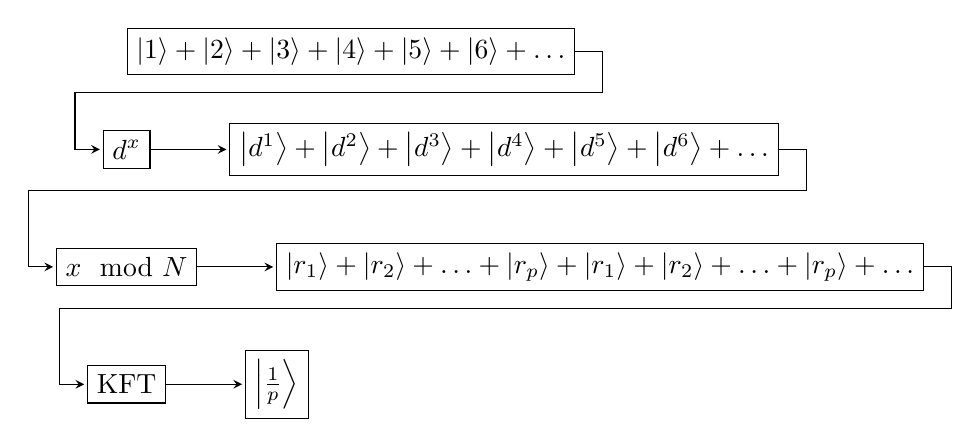
\begin{tikzpicture}[>=stealth,shorten >=1pt]
    \node [draw] (input) {$\left|1\right> + \left|2\right> + \left|3\right> + \left|4\right> + \left|5\right> + \left|6\right> + \ldots $};
    \node [draw, below=of input.west] (step1) {$d^x$};
    \node [draw, right=of step1] (potential) {$\left|d^1\right> + \left|d^2\right> + \left|d^3\right> + \left|d^4\right> + \left|d^5\right> + \left|d^6\right> + \ldots $};
    \node [draw, below=of step1] (mod) {$x\mod N$};
    \node [draw, right=of mod] (mods) {$\left|r_1\right> + \left|r_2\right> + \ldots + \left|r_p\right> + \left|r_1\right> + \left|r_2\right> + \ldots + \left|r_p\right> + \ldots $};

    \path (input.east) ++ (1em,-1.5em) coordinate (input path)
          (step1.west) ++ (-1em,0) coordinate (step1 approach)
          (potential.east) ++ (1em,-1.5em) coordinate (potential path)
          (mod.west) ++ (-1em,0) coordinate (mod approach);


    \draw [->] (input.east) -- (input -| input path) -- (input path) -- (step1 approach |- input path) -- (step1 approach) -- (step1.west);
    \draw [->] (step1) -- (potential);
    \draw [->] (potential.east) -- (potential -| potential path) -- (potential path) -- (mod approach |- potential path) -- (mod approach) -- (mod.west);
    \draw [->] (mod) -- (mods);

    \uncover<2->{
      \node [draw, below=of mod] (qft) {KFT};

      \path (mods.east) ++ (1em, -1.5em) coordinate (mods path)
            (qft.west) ++ (-1em, 0) coordinate (qft approach);

      \draw [->] (mods.east) -- (mods -| mods path) -- (mods path) -- (qft approach |- mods path) -- (qft approach) -- (qft);
    }
    \uncover<3->{
      \node [draw, right=of qft] (result) {$\left|\frac{1}{p}\right>$};
      \draw [->] (qft) -- (result);
    }
  \end{tikzpicture}
  \end{figure}
  \vspace{1em}
  \uncover<2->{\small KFT: kvantuma Fourier transformo}

\end{frame}

\againframe<7>{shor}

\section{Postkvantuma ĉifrado}

\begin{frame}
  \frametitle{Postkvantuma ĉifrado}
  Leviĝas kelkaj demandoj:
  \begin{itemize}
  \item<+-> Ĉu kvantumaj komputiloj realisme povos rompi ĉifrosistemojn?
  \item<+-> Kiam? Ĉu post kvin jaroj? Ĉu post dek? Ĉu post 20?
  \item<+-> Ĉu tio estas problemo?
  \item<+-> Por ŝlosillongeco 4096 oni bezonus 4096 logikajn kubitojn
  \item<+-> Rekorda kvantuma komputilo havas 5000 fizikajn kubitojn
  \end{itemize}

  \vspace{1em}
  \uncover<+->{NIST okazigis konkurson}

  \begin{itemize}
  \item<+-> 69 kandidatoj en 2016
  \item<+-> Post kvar rondoj 4 algoritmoj estis normigataj
  \end{itemize}

  \uncover<+->{%
    \begin{beamercolorbox}[center, rounded=true, shadow=true]{notebox}
      Promesplena: \emph{Crystal KYBER} – laticbazita sistemo
    \end{beamercolorbox}
  }
\end{frame}


\begin{frame}
  \frametitle{Laticbazita ĉifrado}
  Kio estas latico?

  \begin{figure}
  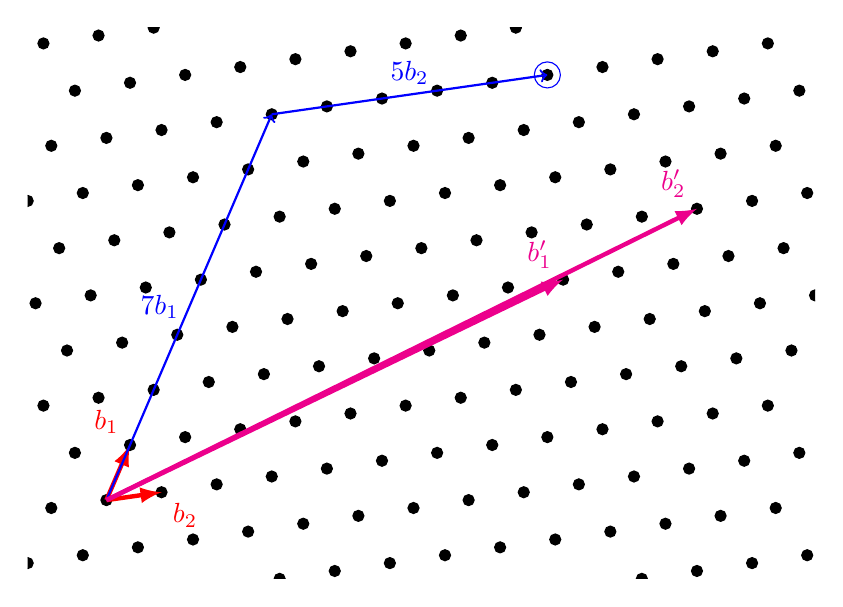
\begin{tikzpicture}
    \coordinate (Origin)   at (0,0);

    \coordinate (Bone) at (0.3,0.7);
    \coordinate (Btwo) at (0.7,0.1);

    % Latice points along b1+b2

    \clip (-1, -1) rectangle (9, 6);

    \foreach \i in {-5, -4, -3, -2, -1, 0, 1, 2, 3, 4, 5, 6, 7, 8, 9, 10} {
      \foreach \j in {-5, -4, -3, -2, -1, 0, 1, 2, 3, 4, 5, 6, 7, 8, 9, 10, 11,
        12, 13 ,14, 15}
        \draw [fill = black]($\i*(Bone)+\j*(Btwo)$) circle (2pt);
    }
    % Draw the vectors
    \draw [ultra thick,-latex,red] (Origin) -- (Bone) node [above left] {$b_1$};
    \draw [ultra thick,-latex,red] (Origin) -- (Btwo) node [below right] {$b_2$};

    \uncover<2->{\node[draw=blue, circle] at ($7*(Bone)+5*(Btwo)$) {};}

    \uncover<3>{
      \draw [thick, blue, ->] (Origin) -- ($7*(Bone)$) node[midway, left] {$7 b_1$};
      \draw [thick, blue, ->] ($7*(Bone)$) -- ++ ($5*(Btwo)$) node[midway, above] {$5 b_2$};
    }

    \only<4->{
      \draw [ultra thick,-latex,magenta] (Origin) -- ($3*(Bone)+7*(Btwo)$) node [above left] {$b'_1$};
      \draw [ultra thick,-latex,magenta] (Origin) -- ($4*(Bone)+9*(Btwo)$) node [above left] {$b'_2$};
    }
  \end{tikzpicture}
  \end{figure}
\end{frame}

\begin{frame}
  \frametitle{Serĉado de plej proksima vektoro}
  \begin{figure}
  \begin{tikzpicture}
    \coordinate (Origin)   at (0,0);

    \coordinate (Bone) at (0.3,0.7);
    \coordinate (Btwo) at (0.7,0.1);

    \coordinate (BoneB) at ($3*(Bone)+7*(Btwo)$);
    \coordinate (BtwoB) at ($4*(Bone)+9*(Btwo)$);

    % Latice points along b1+b2

    \clip (-1, -1) rectangle (9, 4.5);


    \uncover<1-2,9->{
      \foreach \i in {-5, -4, -3, -2, -1, 0, 1, 2, 3, 4, 5, 6, 7, 8, 9, 10} {
        \foreach \j in {-5, -4, -3, -2, -1, 0, 1, 2, 3, 4, 5, 6, 7, 8, 9, 10, 11,
          12, 13 ,14, 15}
        \draw [fill = black]($\i*(Bone)+\j*(Btwo)$) circle (2pt);
      }
    }
    % Draw the vectors
    \only<1-3,8->{
      \draw [ultra thick,-latex,red] (Origin) -- (Bone) node [above left] {$b_1$};
      \draw [ultra thick,-latex,red] (Origin) -- (Btwo) node [below right] {$b_2$};
    }

    \only<2-4>{\draw[fill=blue] ($3.1*(Bone)+4.2*(Btwo)$) circle (2pt);}

    \only<4->{
       \draw [thick,-latex,magenta] (Origin) -- ($3*(Bone)+7*(Btwo)$) node [above left] {$b'_1$};
       \draw [thick,-latex,magenta] (Origin) -- ($4*(Bone)+9*(Btwo)$) node [above left] {$b'_2$};
     }

    \only<5-6,10>{\draw[blue] ($3*(Bone)+4*(Btwo)$) circle (3pt) node [above left] {\color{blue}{$K$}};}
    %\draw [->] (Origin) -- ++ ($-11*(BoneB)+9*(BtwoB)$);
    \only<6->{\draw[fill=blue] ($3.1*(Bone)+4.2*(Btwo)$) circle (2pt) node [above right] {\color{blue}{$M$}};}
  \end{tikzpicture}
  \end{figure}
  \uncover<5-6,10>{%
    \[K = (-11, 9)\]
  }

\end{frame}

\section{Kyber}

\subsection*{Modula aritmetiko}

\begin{frame}
  \frametitle{Entjera ringo}

  Modulo:
  \begin{itemize}
  \item $r = a \mod q$ signifas ke $r$ estas la resto de entjera divido $a/q$.
  \item Entjeraro modulo $q$: $\mathbb{Z}_q = \left\{0, 1, 2, \ldots, q-1\right\}$
  \item Ene de $\mathbb{Z}_q$ ĉia aritmetiko estas farataj $\mod q$.
  \end{itemize}
  \begin{columns}
    \begin{column}<3->{0.5\textwidth}
      Ekzemple por $\mathbb{Z}_{17}$:
      \begin{itemize}
      \item $9 + 15 = 7$
      \item $9 - 15 = 11$
      \item $9 \times 15 = 16$
      \end{itemize}
    \end{column}
    \begin{column}<2->{0.5\textwidth}
      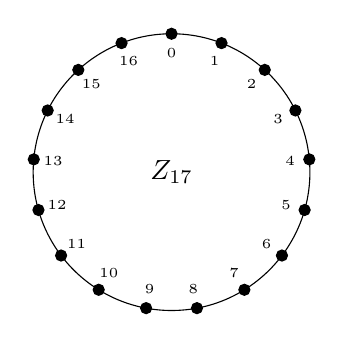
\begin{tikzpicture}
        \draw (0, 0) circle (5em);
        \foreach \n in {0,1,...,16} {%
          \pgfmathparse{-360 * \n / 17 + 90}\edef\a{\pgfmathresult}
          \draw [fill] (\a:5em) circle(2pt);
          \node at (\a:4.3em) {\tiny\n};
        }
        \node at (0, 0) {$\mathbb{Z}_{17}$};
      \end{tikzpicture}
    \end{column}
  \end{columns}
\end{frame}

\begin{frame}
  \frametitle{Polinoma ringo}
  \begin{itemize}
  \item Polinomo $n$-a grada: $c_nx^n + c_{n-1}x^{n-1} + \ldots + c_1 x + c_0$
  \item $\mathbb{Z}_q[x]$: aro de ĉiuj polinomoj kun $c_n \in \mathbb{Z}_q
    \;\forall n$

  \end{itemize}

  \vspace{2em}
  \uncover<2->{Ekzemple $q=7$}
  \begin{itemize}
  \item<3-> $f(x) = 3x^3 + 4x^2 + 5$ kaj $g(x) = 2x^2 + 3x + 6$
  \item<4-> $f(x) + g(x) = 3x^3 + 6x^2 + 3x + 4$
  \item<5-> $f(x) - g(x) = 3x^3 + 2x^2 + 4x + 6$
  \item<6-> $f(x) \times g(x) = 6x^5 + 3x^4 + 2x^3 + 6x^2 + x + 2$
  \end{itemize}

\end{frame}

\begin{frame}
  \frametitle{Polinoma ringo kun limigita grado}
  \[
    R_q = \mathbb{Z}_q[x]/(x^n-1)
  \]

  \begin{itemize}
  \item<+-> $R_q$ estas ĉiuj polinomoj el $\mathbb{Z}_q[x]$ de grado malpli ol $n$
  \item<+-> se $h(x) = f(x) \times g(x)$ havas gradon pli ol $n-1$ ni elektas
    \[h(x) = f(x) \times g(x) \mod (x^n-1)\]
  \end{itemize}

  \vspace{0.5em}
  \uncover<+->{
    Ekzemplo $R_{41} = \mathbb{Z}_{41}[x](x^4-1)$:
    \[
      f(x) = 22x^3 + 17x^2 + 31 \; g(x) = x^3 + 19x^2 + 7x + 11
    \]
    \[
      f(x) \times g(x) = 24x^3 + 35x^2 + 35x + 39
    \]
  }
\end{frame}

\subsection*{Kyber ekzemplo}

\begin{frame}
  \frametitle{Kyber ekzemplo: krei ŝlosilojn}
  Parametroj: $q = 17, \bigl\lfloor\frac{q}{2}\bigr\rceil = 9, \; R_q = \mathbb{Z}_{17}[x](x^4 + 1)$\par
  \pause
  \vspace{0.5em}
  Privata ŝlosilo hazarde elektita
  \[ \mathbf{s} = \left( - 1x^3 - 1x^2 + 1x^1 + 0x^0, - 1x^3 +0x^2 - 1x^1 + 0x^0 \right) \]
  \pause
  Plia datumo hazarde elektita
  \[
    \mathbf{A} =
    \begin{pmatrix}
      6x^3 + 16x^2 + 16x + 11 & 9x^3 + 4x^3 + 6x + 3 \\
      5x^3 + 3x^2 + 10x +1    & 6x^3 + x^2 + 9x + 15
    \end{pmatrix}
  \]
  \[
    \mathbf{e} = \left( x^2, x^2 - x \right)
  \]
  \[
    \mathbf{t} = \mathbf{A}\mathbf{s} + \mathbf{e}
  \]
  \[
    \mathbf{t} = \left( 16x^3 + 15x^2 + 7, 10x^3 + 12x^2 + 11x + 6 \right)
  \]
  \pause
  La publika ŝlosilo konsistas el $(\mathbf{t}, \mathbf{A})$.
\end{frame}

\begin{frame}
  \frametitle{Kyber ekzemplo: ĉifro}
  Ni elektas hazarde:
  \[
    \mathbf{r} = \left( -x^3 + x^2, x^3 + x^2 - 1 \right), \; \mathbf{e_1} = \left( x^2 + x, x^2 \right), \; e_2 = -x^3 - x^2
  \]
  \pause
  Nia mesaĝo estas $11 = (1011)_2$. Kiel polinomo:
  \[m_b = x^3 + x + 1\]
  \pause
  Ni grandigas la polinomon per multobligo kun $\bigl\lfloor\frac{q}{2}\bigr\rceil$:
  \[m = \Bigl\lfloor\frac{q}{2}\Bigr\rceil m_b = 9x^3 + 9x + 9\]
  \pause
  Ni ĉifras:
  \[
    \mathbf{u} = \mathbf{A}^T\mathbf{r} + \mathbf{e_1} \;\text{kaj}\; v = \mathbf{t}^T\mathbf{r} + e_2 + m
  \]
  \pause
  Nia ĉifrita mesaĝo konsistas el
  \[
    \begin{split}
      \mathbf{u} & = (11x^3 + 11x^2 + 10x + 3, 4x^3 + 4x^2 + 13x + 11) \\
      v & = 7x^3 + 6x^2 + 8x + 15
    \end{split}
  \]
\end{frame}

\begin{frame}
  \frametitle{Kyber ekzemplo: malĉifro}
  Ni malĉifras la mesaĝon ricevante mesaĝon kun eraroj:
  \[m_e = v - \mathbf{s}^T\mathbf{u} = 7x^3 + 14x^2 + 7x + 5\]

  \pause
  \begin{columns}
    \begin{column}{0.4\textwidth}
      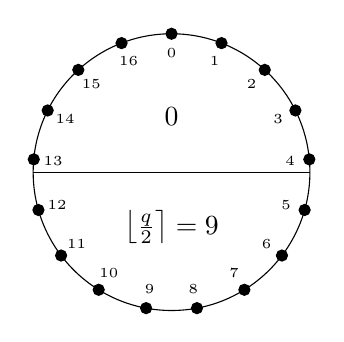
\begin{tikzpicture}
        \draw (0, 0) circle (5em);
        \foreach \n in {0,1,...,16} {%
          \pgfmathparse{-360 * \n / 17 + 90}\edef\a{\pgfmathresult}
          \draw [fill] (\a:5em) circle(2pt);
          \node at (\a:4.3em) {\tiny\n};
        }
        \draw (0:5em) -- (180:5em);

        \node (zero) at (90:2em) {$0$};
        \node (nine) at (270:2em) {$\bigl\lfloor \frac{q}{2} \bigr\rceil = 9$};
      \end{tikzpicture}
    \end{column}

    \begin{column}{0.6\textwidth}
      \[
        \begin{split}
          7 & \longrightarrow 9 \\
          14 & \longrightarrow 0 \\
          7 & \longrightarrow 9 \\
          5 & \longrightarrow 9
        \end{split}
      \]
      \pause
      \[\Longrightarrow m = 9x^3 + 9x + 9\]
      \pause
      \[\Longrightarrow m_b = x^3 + x + 1 \longrightarrow (1011)_2 = 11\]
    \end{column}
  \end{columns}
\end{frame}

\begin{frame}
  \frametitle{Konkludo}
  Kion ni lernis:
  \begin{itemize}
  \item Ĉifrado estas matematiko – pli ekzakte – nombra teorio
  \item Kvantumaj komputiloj ne plu estas matematika modelo
  \item Ekzistas jam ĉifrosistemoj neatakeblaj per kvantumaj komputiloj
  \item<2-> Vivu la matematiko
  \end{itemize}
\end{frame}

\begin{frame}
  \centering Dankon pro la atento
\end{frame}
\end{document}
